\section{Introduction}
In many scientific application domains, the ability to obtain samples from a 
probability distribution is of central interest. 
For instance, sampling methods have been used to discover magnetic polarization 
in the black hole of galaxy M87 \cite{akiyama2021seven}
and to image the Sagittarius A* black hole \cite{akiyama2022first}.
They have also been used to 
model the evolution of single-cell cancer genomes \cite{salehi2021clonal}, 
infer plasma dynamics inside nuclear fusion reactors \cite{gota2021overview}, 
and to identify gerrymandering in Georgia's 2021 congressional districting plan 
\cite{zhao2022mathematically}.
Similarly, evaluating high-dimensional integrals or sums over complicated 
combinatorial spaces are related tasks that can also be solved with sampling 
via Markov chain Monte Carlo (MCMC) methods. 
However, such calculations can often be bottlenecks in the scientific process, with 
simulations that can last days or even weeks to finish. 

\begin{figure}[t]
    \centering
    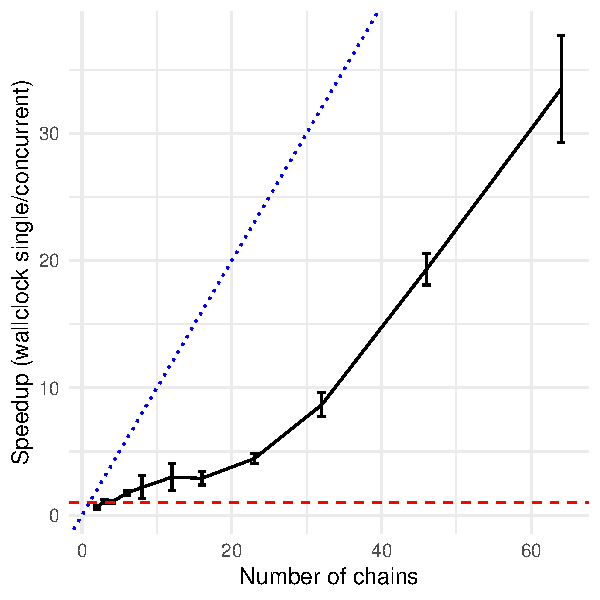
\includegraphics[width=0.7\linewidth]{../img/speedup_distributed.pdf}
%    \hspace{4em}
%    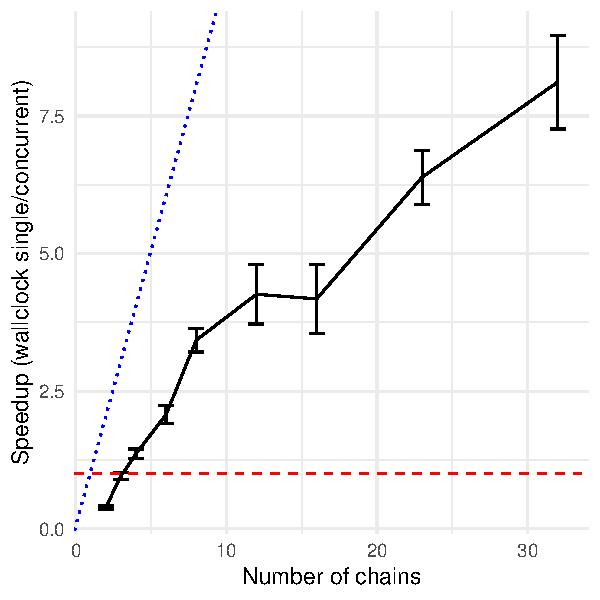
\includegraphics[width=0.33\textwidth]{../img/speedup_parallel.pdf}
    \caption{
        Speedup relative to single-thread execution for Pigeons.jl in the distributed 
        (MPI) setting. Error bars denote approximate 95\% confidence intervals.
        The blue dotted line represents a hypothetical speedup equal to the 
        number of processes. The red dashed line indicates a speedup of one for reference.
    }
    \label{fig:PT_scaling}
\end{figure}

Pigeons.jl\footnote{Documentation available at \url{https://pigeons.run/dev/}. 
Public repository: \url{https://github.com/Julia-Tempering/Pigeons.jl}.}
enables users to sample efficiently from challenging probability distributions.
To achieve this, Pigeons.jl provides a multi-threaded and distributed implementation
of non-reversible \emph{parallel tempering}
(PT; \citealp{syed2021nrpt,syed2021paths,surjanovic2022vpt,surjanovic2024ergodicity}), 
a state-of-the-art MCMC algorithm.
Crucially, Pigeons.jl follows the tuning guidelines described in \citet{syed2021nrpt} 
to provide a hyperparameter-free implementation.
Pigeons.jl's simple user interface facilitates running PT
single-threaded, multi-threaded, and/or distributed over MPI-communicating machines. 
We have stress-tested Pigeons successfully with up to 1,000 processes running 
concurrently on a compute cluster (Sockeye) at the University of British Columbia.
Importantly, Pigeons comes with guarantees on \emph{strong parallelism invariance} (SPI), 
wherein the output for a given seed is \emph{identical} irrespective of the number 
of threads or processes. Such a level of reproducibility is rare in distributed 
software but of great use for the purposes of debugging in the context of sampling 
algorithms, which produce stochastic output.
Specifically, Pigeons.jl is designed to be suitable and yield reproducible output for:
\begin{enumerate}
    \item one machine running on one thread;
    \item one machine running on several threads;
    \item several machines running, each using one thread, and
    \item several machines running, each using several threads.
\end{enumerate}





